\chapter{Using CNN to classify the patches}
Deep learning powers computer vision with processing the data in high level such as image, sound, video in many tasks: classification, recognition or object detection. 
As a result of studying about the CNN, in this chapter, we proposed a model to classify
the landmarks on the pronotum of beetle. For each landmark in pronotum image, a patch
has been extracted with the size of $63\times63$. Then, the patches are used as the input of the model to train. At the end, a number of patches are tested to evaluate
the prediction of the model.

\section{Data}
The pronotum dataset includes 293 images. For each image, a set of 8 landmarks have been set manually by the biologist. For each landmark, a patch is extracted with the size of $63\times63$.
The images have been divided into 3 sets: training set included 200 images ($200 \times 8 = 1600 $ patches), validation set had 60 images ($60 \times 8 = 480$ patches) and 33 images ($33 \times 8 = 264$ patches) belong to the test set.

To evaluate the efficient of the network, the data has been chosen followed 3 ways: 
\begin{enumerate}
	\item In the first way, 200 first images are used as training data; next, 60 images are used as the validation data; and the test is remaining images.
	\item In the second way, 33 first images are chosen as test data; next, 200 and 60 images are chosen as training and validation data, respectively.
	\item In the last way, the images are divided randomly into 3 sets with the corresponding quantity.
\end{enumerate}

Besides, the patch's size also changed to find the suitable size for the patch for each landmark: $27 \times 27$, $45 \times 45$ and $63 \times 63$. The network trained with two types of the images: grayscale and RGB color.
\section{The network}
We propose a CNN-based method to classify the landmarks on the pronotum (see Fig. \ref{figCNNclassify}). The input of the network is the patches around the landmarks. The network includes three convolutional (CONV) layers followed by three pooling layers (maximum and average pooling) and two full connected layers. 
\begin{figure}[h]
	\centering
	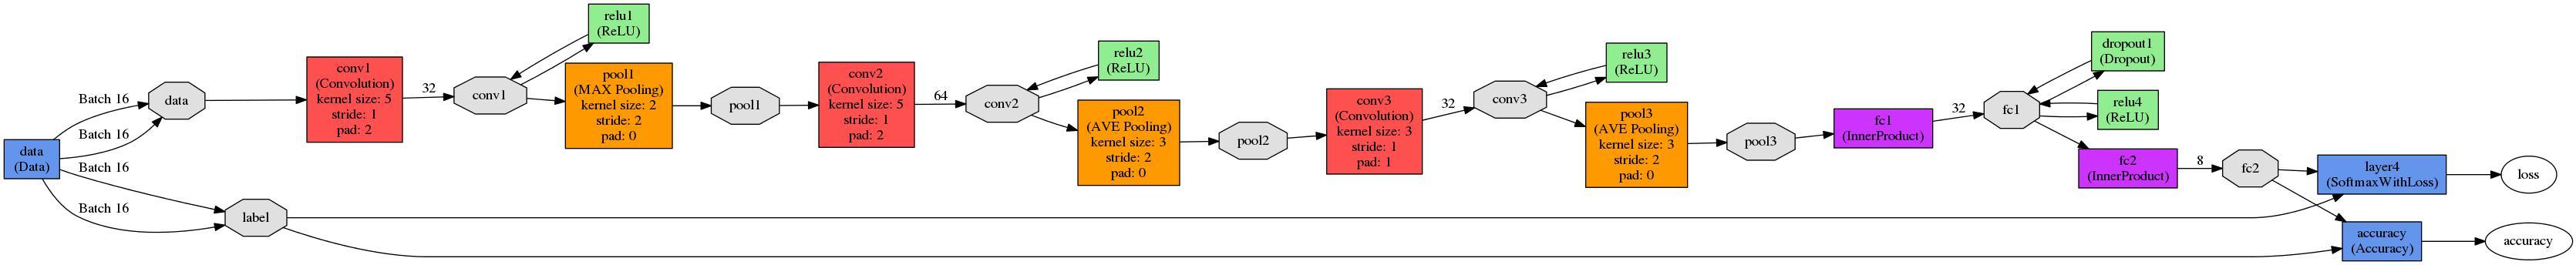
\includegraphics[scale=0.2]{images/CNN_classify}
	\caption{CNN model architecture}
	\label{figCNNclassify}
\end{figure}

The number of convolution filters are 32, 64 and 32, respectively. The window size of those filters are $5\times5, 5\times5$ and $3\times3$. For each CONV layer, a Rectifier Linear Unit is add to introduce the non-linearity for CNN.

Followed each CONV layer is a pooling (POOL) layer. The POOL layers with stride of $2\times2$ is reducing the computation for the deeper layers. The first fully connected (FC) layer consists of 32 neurons. To reduce the risk of the over-fitting on the network, a dropout layer is followed the first FC. The second FC layer output 8 values corresponding to 8 classes of the landmarks. Finally, a softmax with loss layer and accuracy layer are placed at the last stage of the network.
\section{Solver parameters}
The network is trained in $100000$ iterations. For each $10000$ iterations, a test phase will be executed in $1200$ iterations to validate the accuracy of the network.
During training, the Stochastic Gradient Descent (SGD) is used to update the value for learnable parameters. At the beginning, the learning rate is set to $0.0001$, after each $22000$ iterations, the learning rate is dropped as $10^{-3}$. Besides, $90\%$ value of previous computation will be retained in the new calculation.
\section{Experiment and results}
The network is trained with the data that chosen in three ways. In each way, two kinds of datasets are used: color patches and grayscale patches. For each dataset, three patch's size is used to prepare the data: $27\times27$, $ 45\times45$ and $63\times63$. The accuracy of the network on each dataset is provided in the tables following:
\begin{table}[h]
	\centering
	\begin{tabular}{{l}*{3}{c}}
		
		Size of patches &  $27 \times 27$ & $ 45 \times 45$ & $63 \times 63$  \\ \hline
		Accuracy on color patches & 73 & 83.14 & 88.97 \\ 
		Accuracy on grayscale patches & 57.25 & 72.08 & 77.91 \\ 
		\hline
	\end{tabular}
	\caption{The accuracy of the model on the data that chosen by the first way.}
	\label{tb1}
\end{table}

\begin{table}[h]
	\centering
	\begin{tabular}{{l}*{3}{c}}
		
		Size of patches &  $27 \times 27$ & $ 45 \times 45$ & $63 \times 63$  \\ \hline
		Accuracy on color patches & 75.193 & 85.417 & 89.168 \\ 
		Accuracy on grayscale patches & 64.385 & 72.11 & 78.1077 \\ 
		\hline
	\end{tabular}
	\caption{The accuracy of the model on the data that chosen by the second way.}
	\label{tb2}
\end{table}

\begin{table}[h]
	\centering
	\begin{tabular}{{l}*{3}{c}}
		
		Size of patches &  $27 \times 27$ & $ 45 \times 45$ & $63 \times 63$  \\ \hline
		Accuracy on color patches & 77.286 & 87.751 & 89.979 \\ 
		Accuracy on grayscale patches & 64.163 & 76.455 & 82.709 \\ 
		\hline
	\end{tabular}
	\caption{The accuracy of the model on the data that chosen by the third way.}
	\label{tb3}
\end{table}
As the result shown in three tables (table. \ref{tb1}, \ref{tb2}, \ref{tb3}), it seems that the network did not have more sensitive with the way to choose the data. But we have the different result from color and grayscale patches and the result is also improved when we increase the size of the patches from $27\times27$ to $63\times63$.

From the accuracy of training on each dataset, the patches of size $63\times63$ which selected by randomly are used to predict. The prediction is run on $33$ images ($33 \times 8 = 264$ patches). The label of a patch is label with highest prediction. Table \ref{tb4} shows the statistic of prediction on the dataset. Followed that, most of the landmarks are predicted with high accuracy ($\geq 78\%$). The proportion on $5^{th}$ landmark is not hight and it has a confusion with the $1^{st}$ landmark.
\begin{table}
	\centering
	\begin{tabular}{*{9}{c}}
		& LM 1 & LM 2 & LM 3 & LM 4 & LM 5 & LM 6 & LM 7 & LM 8 \\ \hline
		LM 1 & 87.88\% & 	6.06\% &	 0.00\% &	0.00\% & 	0.00\% & 	0.00\% & 	0.00\%	& 6.06\% \\ \hline
		LM 2 &	6.06\% &	 	90.91\% &	3.03\% & 	0.00\% & 	0.00\% & 	0.00\% & 	0.00\% & 	0.00\% \\ \hline
	LM 3 &	0.00\% & 	3.03\% & 	87.88\% &	3.03\% & 	0.00\% & 	0.00\% & 	6.06\% & 	0.00\% \\ \hline
	LM 4	 & 9.09\% &	0.00\% & 	6.06\% & 	81.82\% &	0.00\% & 	0.00\% & 	3.03\% & 	0.00\% \\ \hline
	LM 5	 & 51.52\% &	0.00\%	& 0.00\%	 & 9.09\% &	39.39\%	& 0.00\%	 & 0.00\% &	0.00\% \\ \hline
	LM 6	 & 12.12\%	& 3.03\%	 & 0.00\% &	0.00\% & 	0.00\% & 	81.82\% &	0.00\% & 	3.03\% \\ \hline
	LM 7	 & 3.03\%	& 0.00\%	 & 9.09\%	& 0.00\%	 & 0.00\%	& 0.00\%	 & 84.85\% &	3.03\% \\ \hline
	LM 8	 & 18.18\%	& 0.00\% &	0.00\%	& 0.00\%	 & 0.00\%	& 0.00\% &	3.03\% &	78.79\% \\ \hline

	\end{tabular}
	\caption{The prediction accuracy on the color patches of size $63\times63$}
	\label{tb4}
\end{table}
\section{Conclusion}
In the content of this work, a model in CNN is proposed to predict the class of the landmarks on pronotum. The network consist 8 layers: 3 CONVs, 3 POOL, 2 FC. For each landmark, the patches with different size are extracted to use as the input data of the model. The experiment shown that the model is worked well on the color batches with larger size. However, a confusion also exists when the model try to predict $5^{th}$ landmark.